% -----------------------------------------------------------------
% 			  Modellbildung und Systemidentifikation
% -----------------------------------------------------------------
% \section*{Modellbildung und Systemidentifikation}

\section*{Introduction}
Euklidische Norm: 
\begin{equation*}
{ \parallel x\parallel  }_{ 2 }\quad =\quad \sqrt { \sum _{ i=1 }^{ n }{ { x }_{ i }^{ 2 } }  } \quad =\quad \sqrt { { x }^{ T }x }
\end{equation*}
\begin{equation*}
{\parallel x\parallel  }_{ 2 }^{ 2 } = x^T\cdot x
\end{equation*}
Weighting Eukledian Norm:
\begin{equation*}
{\parallel x\parallel  }_{ Q }^{ 2 } = x^TQ \cdot x
\end{equation*}
Frobenius Norm:
\begin{equation*}
{\parallel x\parallel  }_{ F }^{ 2 } = trace(A{ A }^{ T })=\sum _{ i=1 }^{ n } \sum _{ j=1 }^{ m }{ { A }_{ ij }{ A }_{ ij } } 
\end{equation*}
\begin{equation*}
\triangledown f(x) \quad Jacobian
\end{equation*}
\begin{equation*}
{ \triangledown  }^{ 2 }f(x)\quad Hessian
\end{equation*}
Error in variables
\begin{equation*}
\hat { R } _{ ev }(N)\quad =\quad \frac { \frac { 1 }{ N } \sum _{ k=1 }^{ N }{ u(k) }  }{ \frac { 1 }{ N } \sum _{ k=1 }^{ N }{ i(k) }  }
\end{equation*}
Matrix derivatives
\begin{equation*}
\frac{d(c^Tx)}{dx} = c
\end{equation*} 
\begin{equation*}
\frac{d(x^TAx)}{dx} = (A^T + A)x
\end{equation*} 
Linear and non-linear equations:
TODO; polynomial etc. 

% -----------------------------------------------------------------
% 				   Probablility and Statistics
% -----------------------------------------------------------------
\section*{Probablility and Statistics}
Random Variables and Probability
\begin{equation*}
P(A|B) \cdot  P(B) = P(B|A) \cdot  P(A)
\end{equation*}
\begin{equation*}
P(A|B) = \frac { P(A,B) }{ P(B) }  \rightarrow  \frac { P(B,A) \cdot  P(A) }{ P(B) } 
\end{equation*}
\begin{equation*}
P(X \in  [a,b]) = \int _{ a }^{ b }{  p_{ X }(x) dx } 
\end{equation*}
Mean
\begin{equation*}
\mu_X = \mathbb{ E }\{ f(x)\}  := \int _{ -\infty  }^{ \infty  }{  f(x) \cdot  p_{ X }(x) dx } 
\end{equation*}
\begin{equation*}
\mathbb{ E }\{ a + bX\}  := a + b\mathbb{ E }\{ X\} 
\end{equation*}
Variance
\begin{equation*}
\sigma _{ X }^{ 2 } := \mathbb{ E }\{ (X-\mu _{ X })^{ 2 }\}  = \mathbb{ E }\{ X^{ 2 }\} -\mu _{ X }^{ 2 }
\end{equation*}
\begin{equation*}
std dev \, \sigma _{ X } = \sqrt { variance \, \sigma _{ X }^{ 2 } } 
\end{equation*}
\section*{Distributions}
Uniform distribution:
\begin{equation*}
{ P_{ y }(x) } = \left\{ \begin{matrix} \frac { 1 }{ b-a }  &  \quad if\quad x  \in  [a,b] \\ 0 & else \end{matrix} \right.
\end{equation*}
Normal (Gaussian) distribution:
\begin{equation*}
p(x) = \frac{1}{\sqrt{2\pi \sigma^2}}\cdot exp(-\frac{(x-\mu)^2}{2\sigma^2})
\end{equation*}
\begin{equation*}
X \sim \mathcal{N}(\mu, \sigma^2)
\end{equation*}
Multidimensional Normal Distribution:
\begin{equation*}
p(x)=\frac { 1 }{ \sqrt { (2\pi )^{ n }\cdot det(\Sigma ) }  } \cdot exp(-\frac { 1 }{ 2 } \, \cdot \, { (x-\mu ) }^{ T }\, \cdot \, \Sigma ^{ -1 }\, \cdot \, (x-\mu )\, )
\end{equation*}
Weibull distribuation: 
\begin{equation*}
F(x) \, = \, 1 - e^{-(\lambda \cdot x)^k}
\end{equation*}
Laplace distribuation:
\begin{equation*}
f(x|\mu,b) = \frac{1}{2b} \cdot exp (-\frac{|x-\mu|}{b})
\end{equation*}
Covariance and Correlaton:
\begin{equation*}
\sigma (Y,Z) := \mathbb{E} {(Y-\mu_Y)(Z-\mu_Z)} = 
\end{equation*}
\begin{equation*}
= \int_{-\infty}^{\infty}{\int_{-\infty}^{\infty}{(y-\mu_Y)(z - \mu_Z)\cdot p_{Y,Z} (y,z)\,  dy \, dz} }
\end{equation*}
Multidimensional Random Variables:
\begin{equation*}
\mathbb{E}{f(X)} = \int_{\mathbb{R}^n}{f(x)p_X(x) d^n x}
\end{equation*}
\begin{equation*}
cov(X) = \mathbb{E} \{(X-\mu_X)(X-\mu_X)^T\} 
\end{equation*}
\begin{equation*}
cov(X) = \mathbb{E} \{XX^T\} - \mu_X \mu_X^T
\end{equation*}
\begin{equation*}
cov(Y) = \Sigma_y = A \Sigma_x A^T \quad for \quad y = A \cdot x
\end{equation*}
\begin{equation*}
\mathbb{E }\{AX\} =A \cdot \mathbb{ E }\{X\}
\end{equation*}
Rules for variance:
\begin{equation*}
var(X+Y) = var(X)+var(Y)+2 \cdot cov(X,Y)
\end{equation*}
\begin{equation*}
var(aX) = {a}^{2} \cdot var(X)
\end{equation*}
Verschiebesatz:
\begin{equation*}
var(X)={ { \mathbb{E}((X-\mathbb{E}(X)) }^{ 2 } })=\mathbb{E}({ X }^{ 2 })-{ (\mathbb{E}(X)) }^{ 2 }
\end{equation*}

unit Variance is variance = 1

Statistical estimators:\\
\textbf{Biased- and unbiasedness} $\rightarrow$ an estimator ${\hat{\theta}}_{N}$ is called unbiased iff $\mathbb{E}\{ {\hat{\theta}}_{N} ({y}_{N})\} = \theta_0$, where ${\theta}_{0}$ is the true value of a parameter. Otherwise, is called biased.

\textbf{Asymptotic Unbiasedness} $\rightarrow$ An estimator ${\hat{\theta}}_{N}$ is called asymptotically unbiased iff 
$
\lim\limits_{n \to \infty} \mathbb{E}\{ {\hat{\theta}}_{N} ({y}_{N}) \} = \theta_0
$

\textbf{Consistency} $\rightarrow$ An estimator ${\hat{\theta}}_{N} ({y}_{N})$ is called consistent if, for any $ \epsilon > 0$, the probability $
P( {\hat{\theta}}_{N} ({y}_{N}) \in [\theta_0 - \epsilon, \theta_0 + \epsilon])
$ tends to one as $N \rightarrow \infty$.


\newpage
\section*{Unconstrainded Optimization}
\textbf{Theorem 1} (First Order Necessary Conditions)\\
If $x^* \in D$ is local minimizer of $f : D \rightarrow \mathbb{R}$ and $f \in C^1$ then
$\triangledown f (x^*) = 0$
Definition (Stationary Point) A point $\bar{x}$ with $\triangledown f(\bar{x}) = 0$ is called a stationary point of f.

\textbf{Theorem 2} (Second Order Necessary Conditions)\\
If $x^* \in D$ is local minimizer of $f : D \rightarrow R$ and $f \in C^2$ then
$\triangledown^2 f(x^*) \succeq 0$

\textbf{Theorem 3} (Second Order Sufficient Conditions and Stability under Perturbations)\\
Assume that $f : D \rightarrow R$ is $C^2.$ If $x^* \in D$ is a stationary point and
$ \triangledown^2 f(x^*) \succ 0$
then $x^*$ is a strict local minimizer of f. In addition, this minimizer is locally unique and is stable against small perturbations of f, i.e. there exists a constant C such that for sufficiently small $p \in \mathbb{R}^n$ holds\\
\begin{equation*}
\parallel{x^* - arg\, \underset{x}{min}  (f(x) + p^T x)}\parallel \,\, \leq \, C\parallel{p}\parallel
\end{equation*}



% -----------------------------------------------------------------
% 				 Linear Least Squares Estimation
% -----------------------------------------------------------------
\section*{Linear Least Squares Estimation}
Preliminaries: I.I.D and gaussian noise

Overall Model
\begin{equation*}
y(k)={ \phi (k) }^{ T }\theta +\epsilon (k)
\end{equation*}

Least Squares cost function as sum
\begin{equation*}
\sum _{ k=1 }^{ N }{{ (y(k)-{ \phi (k) }^{ T }\theta )}^{2  } } 
\end{equation*}

Least Squares cost function
\begin{equation*}
f(\theta )={ \parallel {y  }_{N  }-{ \Phi }_{ N }\theta\parallel }_{ 2 }^{2  }
\end{equation*}

Unique minimizers
\begin{equation*}
\hat{\theta}_{LS} =arg \, \underset{ \theta \in \mathbb{R} }{ min } \, f(\theta)
\end{equation*}

\begin{equation*}
{ \theta  }^{ * }=\underbrace { { ({ \Phi  }^{ T }\Phi ) }^{ -1 }{ \Phi  }^{ T } }_{ { \Phi  }^{ + } } y
\end{equation*}
Pseudo Inverse: \qquad $\Phi ^{ + }={({ \Phi  }^{ T }\Phi ) }^{ -1 }{ \Phi  }^{ T }$\\

Weighted Least Squares (unitless)\\
For I.I.D noise: Unweight Least Squares is optimal: W=I
\begin{equation*}
\sum _{ k=1 }^{ N }\frac {{{ (y(k)-{ \phi (k) }^{ T }\theta )}^{2  } }}{\sigma_{\epsilon}^{2}(k)}
\end{equation*}


\begin{equation*}
{ f }_{ WLS }(\theta )={ \parallel { y }_{ N }-{ \Phi  }_{ N }\theta \parallel  }_{ W }^{ 2 }={ ({ Y }_{ N }-\Phi \cdot \theta ) }^{ T }\cdot W\cdot  ({ Y }_{ N }-\Phi \cdot \theta )
\end{equation*}




\begin{equation*}
{ \hat{\theta} }_{ WLS }=arg\, \underset{ \theta \in \mathbb{R} }{ min }\,{f  }_{WLS  }(\theta)={ ({\Phi}^{T}W\Phi) }^{ -1 }{\Phi}^{T} Wy
\end{equation*}


Singular Value Decomposition
\begin{equation*}
A=US{ V }^{ T }\quad mit\quad U\in\mathbb{{R}}^{mxm}, \quad V\in\mathbb{{R}}^{nxn} und \quad S\in\mathbb{{R}}^{mxn}
\end{equation*}

Moore Penrose Pseudo Inverse
\begin{equation*}
{ \Phi  }^{ + }=V{ S }^{+}{U}^{T}
\end{equation*}

Regularization for Least Squares\\
\( { lim }_{ \alpha \rightarrow 0 }{ ({ \Phi  }^{ T }\Phi +\alpha { I }) }^{ -1 }{ \Phi  }^{ T }={ \Phi  }^{ + }\, with\,{ \Phi  }^{ + }\, MPPI \)
\begin{equation*}
{ \theta  }^{ * }(\alpha )=arg\, \underset { \theta \in { R } }{ min } \, \frac { 1 }{ 2 } {\parallel y-\Phi\theta \parallel}_{2}^{2}+\frac { \alpha }{ 2 } {\parallel \theta\parallel}_{2}^{2}
\end{equation*}

Expectation of Least Squares Estimator
\begin{equation*}
{ E }\{ { \hat { \theta  } _{ WLS } }\} { ={ E }\{ ({ \Phi  }_{ N }^{ T }W{ \Phi  }_{ N }) }^{ -1 }{ \Phi  }_{ N }^{ T }W{ y }_{ N }\} ={\theta}_{0}
\end{equation*}


Covariance of the least squares estimator
\begin{equation*}
cov({ \hat { \theta  } _{ WLS } }){ =({ \Phi  }_{ N }^{ T }W{ \Phi  }_{ N }) }^{ -1 }{ =({ \Phi  }_{ N }^{ T }{\Sigma}_{\in N }^{ -1 }{ \Phi  }_{ N }) }^{ -1 }
\end{equation*}

\begin{equation*}
cov({ \hat { \theta  } _{ WLS } }){ \succeq ({ \Phi  }_{ N }^{ T }W{ \Phi  }_{ N }) }^{ -1 }
\end{equation*}


Example:
\begin{equation*}
\varepsilon (1) \sim  { \cal{N} }(0|\sigma ^{ 2 }_{ 1 }) \quad \varepsilon (2) \sim  { \cal{N} }(0|\sigma ^{ 2 }_{ 2 })
\end{equation*}

\begin{equation*}
N=2 \quad { \Sigma  }_{ { \varepsilon  }_{ N } }=\quad \begin{bmatrix} \sigma _{ 1 }^{ 2 } & 0 \\ 0 & \sigma _{ 2 }^{ 2 } \end{bmatrix}
\end{equation*}

\begin{equation*}
W^{ OPT } = \Sigma _{ ^{ \varepsilon_{ N } } }^{ -1 }\quad \begin{bmatrix} \frac { 1 }{ \sigma _{ 1 }^{ 2 } }  & 0 \\ 0 & \frac { 1 }{ \sigma _{ 2 }^{ 2 } }  \end{bmatrix}
\end{equation*}

\begin{equation*}
cov({ \hat { \theta  } _{ WLS } }){ =({ Y }_{ N }-{ \Phi  }_{ N }\theta ) }^{ T }\cdot W\cdot ({ Y }_{ N }-{ \Phi  }_{ N }\theta )=
\end{equation*}

\begin{equation*}
\sum _{ k=1 }^{ 2 }{ (y(k)-{ \phi (k) }^{ T }\theta )\cdot \frac { 1 }{ { \sigma  }_{ k }^{ 2 } } \cdot (y(k)-{ \phi (k) }^{ T }\theta ) } 
\end{equation*}


Measuring the goodness of Fit using \({R}^{2} \quad 0\le {R}^{2} \le1\) 
\begin{equation*}
{ R }^{ 2 }=1-\frac { { \parallel { y }_{ N }-{ \Phi  }_{ N }\hat { \theta  } \parallel  }_{ 2 }^{ 2 } }{ { \parallel { y }_{ N }\parallel  }_{ 2 }^{ 2 } } =1-\frac { { \parallel { \epsilon  }_{ N }\parallel  }_{ 2 }^{ 2 } }{ { \parallel { y }_{ N }\parallel  }_{ 2 }^{ 2 } } =
\end{equation*}
\begin{equation*}
\frac { { \parallel { y }_{ N }\parallel  }_{ 2 }^{ 2 }-{ \parallel { \epsilon  }_{ N }\parallel  }_{ 2 }^{ 2 } }{ { \parallel { y }_{ N }\parallel  }_{ 2 }^{ 2 } } =\frac { { \parallel { \hat { y  }  }_{ N }\parallel  }_{ 2 }^{ 2 } }{ { \parallel { y }_{ N }\parallel  }_{ 2 }^{ 2 } } 
\end{equation*}
residual $ \epsilon_{N} \uparrow \quad \rightarrow \quad R^{2} \rightarrow 0 \,\,(= bad)$





Estimating the Covariance with the Single Experiment
\begin{equation*}
\hat { \sigma  } _{ \varepsilon  }^{ 2 } := \frac { 1 }{ N-d } \sum _{ k=1 }^{ N }{ (y(k)-\phi (k)^{ T }\hat { \theta  } _{ LS })^{ 2 } }  = \frac { \parallel y_{ N }-\phi _{ N }\hat { \theta  } _{ LS }{ \parallel  }_{ 2 }^{ 2 } }{ N-d } 
\end{equation*}

\begin{equation*}
\hat { \Sigma  } _{ \hat { \theta  }  } := \hat { \sigma  } ^{ 2 }_{ \varepsilon  } (\phi ^{ T }_{ N } \phi _{ N })^{ -1 } = \frac { \parallel y_{ N }\, -\phi _{ N }\hat { \theta  } _{ LS }{ \parallel  }_{ 2 }^{ 2 } }{ N-d } \cdot (\phi ^{ T }_{ N } \phi _{ N })^{ -1 }
\end{equation*}



\newpage
% -----------------------------------------------------------------
% 				 Maximum Likelihood Estimation
% -----------------------------------------------------------------
\section*{Maximum Likelihood Estimation}
Maximum Likelihood Estimation (ML) \({L}_{2}\) Estimation:\\
Measurement Errors assumed to be Normally distributed
\begin{equation*}
{ P(y|\theta ) }=C\prod _{ i=1 }^{ N }{ exp(\frac { -(y_{ i }-M_{ i }(\theta ))^{ 2 } }{ 2\cdot \sigma _{ i }^{ 2 } } )} 
\end{equation*}

Positive log-Likelihood. Logarithm makes from products a sum!
\begin{equation*}
{ log \, p(y|\theta ) } = log(C) +\sum _{ i=1 }^{ N }{ { \frac { -(y_{ i }-M_{ i }(\theta ))^{ 2 } }{ 2 \cdot \sigma _{ i }^{ 2 } }  } } 
\end{equation*}

Negative log-Likelihood:
\begin{equation*}
\hat{\theta}_{ML} \, = \, arg \, \underset { \theta \in { \mathbb{R} }^{ d } }{ max } \, p(y|\theta ) = arg \, \underset { \theta \in { \mathbb{R} }^{ d } }{ min }  \sum _{ i=1 }^{ m }{ \frac { (y_{ i }-M_{ i }(\theta ))^{ 2 } }{ 2\, { \sigma _{ i } }^{ 2 } }  } 
\end{equation*}

\begin{equation*}
arg \, \underset{ \theta \in \mathbb{ R }^{ d } }{ max } \, p(y|\theta ) = arg \, \underset { \theta \in {  R }^{ d } }{ min } \quad \frac{1}{2} \parallel S^{ -1 }\cdot (y-M(\theta )){ \parallel  }_{ 2 }^{ 2 }
\end{equation*}

\({L}_{1}\) Estimation:\\
Measurement Errors assumed to be Laplace distributed.\\ \(Median(x)=\left\lceil \frac { x + 1 }{ 2 }  \right\rceil \)\\
Robust against outliers
\begin{equation*}
\underset { \theta  }{ min } { \parallel y-M(\theta )\parallel  }_{ 1 }\,=\,\underset { \theta  }{ min } \sum _{ i=1 }^{ N }{ |{ y }_{ i }-{ M }_{ i }\theta | } \,=
\end{equation*}
\begin{equation*}
=\,median\,of\,\{{Y}_{1},...,{Y}_{N}\}
\end{equation*}



\begin{equation*}
{ P(y|\theta ) }=C\prod _{ i=1 }^{ N }{ { exp }(\frac { -|{ y }_{ i }-\theta | }{ 2\cdot { a }_{ i } } ) } 
\end{equation*} 

Bayesian Estimation and the Maximum a Posteriori Estimate\\
Assumptions: i.i.d noise and linear model
\begin{equation*}
p(\theta |{ y }_{ N })\cdot p({ y }_{ N })=p({ y }_{ N }|\theta )\cdot p(\theta)
\end{equation*}

\begin{equation*}
{ \hat{\theta} }_{ MAP } = arg \, \underset { \theta \in \mathbb{R} }{ min } \{-log(p({ y }_{ N }|\theta))-log(p(\theta))\}
\end{equation*}

MAP Example: Regularised Least Squares
\begin{equation*}
\theta =\overline { \theta  } \pm { \sigma  }_{ \theta  }\quad with \quad \overline { \theta  } = { \theta  }_{ apriori  }
\end{equation*}

\begin{equation*}
{ \hat { \theta  }  }_{ MAP }=arg\, \underset { \theta \in { R } }{ min } \frac { 1 }{ 2 } \cdot \frac { 1 }{ { \sigma  }_{ \epsilon  }^{ 2 } } \cdot { \parallel { y }_{ N }-{ \Phi  }_{ N }\cdot \theta \parallel  }_{ 2 }^{ 2 }+\frac { 1 }{ 2 } \cdot \frac { 1 }{ { \sigma  }_{ \theta  }^{ 2 } } \cdot { (\theta -  \overline{\theta}) }^{ 2 }
\end{equation*}

\subsection*{Recursive Linear Least Squares}
\begin{equation*}
\theta _{ ML }(N) \, = \, arg\, \underset { \theta \, \in \, { R } }{ min } \, \frac { 1 }{ 2 } \parallel y_N - \Phi_N\cdot\,\theta{ \parallel  }_{ 2 }^{ 2 }
\end{equation*}

\begin{equation*}
\hat { \theta  } _{ ML }\, (N+1)\, =\, arg\, \underset { \theta \, \in \, { R^{ d } } }{ min } \, (\alpha \, \cdot \, \frac { 1 }{ 2 } \, \cdot \, \parallel \theta \, - \, \hat { \theta  } _{ ML }(N){ \parallel  }_{ Q_{ N } }^{ 2 }+
\end{equation*}
\begin{equation*}
\frac { 1 }{ 2 } \, \cdot \, \parallel y(N+1) \, - \, \varphi (N+1)^{ T }\, \cdot \, \theta \, { \parallel  }_{ 2 }^{ 2 })
\end{equation*}

\begin{equation*}
Q_{ 0 }\quad given,\quad and\quad \hat { \theta  } _{ ML }(0)\quad given,
\end{equation*}
\begin{equation*}
Q_{ N+1 }\, =\, \alpha \, \cdot \, Q_{ N }+\varphi (N+1)\, \cdot \, \varphi (N+1)^{ T },
\end{equation*}
\begin{equation*}
\hat { \theta  } _{ ML }(N+1)\, =\, \hat { \theta  } _{ ML }(N)+Q_{ N+1 }^{ -1 }\, \cdot \, \varphi (N+1)\, \cdot \, [y(N+1)-
\end{equation*}
\begin{equation*}
\varphi(N+1)^T \, \cdot \,\hat{\theta}_{ML}(N)]
\end{equation*}

\subsection*{Cramer-Rao-Inequality}
\begin{equation*}
{ \Sigma  }_{ \theta  } \succeq M^{-1} = (\Phi^T_N \cdot \Sigma^{-1} \cdot \Phi)^{-1}
\end{equation*}
\begin{equation*}
L(\theta ,y_{ N })\, =\, \frac { 1 }{ 2 } \, \cdot \, (\Phi _{ N }\, \cdot \, \theta \, -\, y_N)^{ T } \, \cdot \, \Sigma^{-1} \, \cdot \,  (\Phi_N \, \cdot \, \theta \, - \, y_N) =log\, (p({ y }_{ N }|\theta))
\end{equation*}
\begin{equation*}
M\, =\, { E }\{ \triangledown ^{ 2 }_{ \theta  }\, L(\theta ,y_{ N })\} \, =\, \triangledown ^{ 2 }_{ \theta  }\, L(\theta ,y_{ N })\, =\, \Phi _{ N }^{ T }\, \cdot \, \Sigma ^{ -1 }\, \cdot \, \Phi _{ N }
\end{equation*}

% -----------------------------------------------------------------
%		 				 Dynamic Models
% -----------------------------------------------------------------
\section*{Dynamic Models}
\textbf{Linear Time Invariant (LTI) Systems}\\
with A, B, C, D are matrices
\begin{equation*}
\dot { x } =Ax+Bu \quad y=Cx+Du 
\end{equation*}
\begin{equation*}
G(s)=C{ (sI-A) }^{ -1 }B+D
\end{equation*}

LTI sytems as Input-Output Models
\begin{equation*}
G(S)\, =\, \frac { b_0 + b_1s+...+b_ns^n }{ a_0+a_1s+...+a_{n-1}s^{n-1}+s^n } 
\end{equation*}

\textbf{Different Models}\\
\textbf{Deterministic Model:} \(y(k)=M(k;U,{ x }_{ init },p)\) \\
\textbf{Model with measurement Noise:} \\ \(y(k)=M(k;U,{ x }_{ init },p)+\varepsilon(k)\) \\
\textbf{Model with Input and Output Errors:} \\ \( \quad y(k)=M(k;U+{\varepsilon  }_{ N }^{ u },{ x }_{ init },p)+{ { \varepsilon }^{ y } }(k)\)


Pure Output Error (OE) Minimization
\begin{equation*}
\theta _{ ML } \, =\, arg\, \underset { \theta  }{ min } \, \sum _{ k=1 }^{ N }{ (y(k)-M(k;U,\, x_{ init }\, ,\, p)\, )^{ 2 } }
\end{equation*}

Output Error Minimization for FIR Models
\begin{equation*}
y(k) \, = \, (u(k),\, u(k-1),\, ...,\, u(k-n_{n_b})) \, \cdot \, \theta \, + \, \varepsilon(k)
\end{equation*}

\begin{equation*}
\underset { \theta  }{ min } \sum _{ k=n_{ b }+1 }^{ N }{ (\quad y(k)\, -\, (u(k),\, u(k-1),\, ...,\, u(k-n_{ n_{ b } }))\, \cdot \, \theta \quad )^{ 2 } } 
\end{equation*}


\begin{figure}[H]
	\centering
  	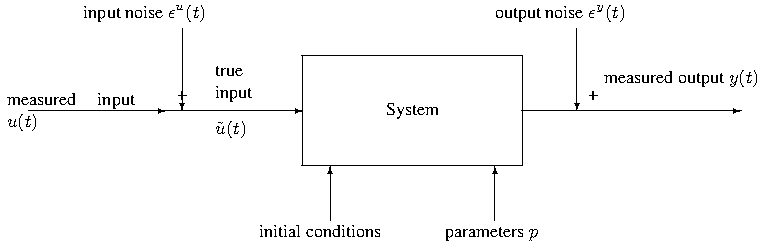
\includegraphics[width=0.5\textwidth]{./model.pdf}
	\label{model}
\end{figure}
Models with Input and Output Errors
\begin{equation*}
arg \, \underset { \theta  }{ min } \, \sum _{ k-1 }^{ N }{ \frac { 1 }{ { \sigma  }_{ y }^{ 2 } }  } { (y(k)-M(k;U+{ \epsilon  }_{ N }^{ u },{ x }_{ init },p)) }^{ 2 }+\frac { 1 }{ { \sigma  }_{ u }^{ 2 } } { ({ \epsilon  }_{ u }(k)) }^{ 2 }
\end{equation*}


\begin{equation*}
arg \, \underset { \theta  }{ min } \, \sum _{ k-1 }^{ N }{ \frac { 1 }{ { \sigma  }_{ y }^{ 2 } }  } { (y(k)-M(k;\tilde { U } ,{ x }_{ init },p)) }^{ 2 }+\frac { 1 }{ { \sigma  }_{ u }^{ 2 } } { (u(k)-\tilde{ u }(k) ) }^{ 2 }
\end{equation*}





\newpage
% -----------------------------------------------------------------
%	 Non parametric and frequency domain identification methods
% -----------------------------------------------------------------
\section*{Fourier Transformation}
\textbf{How to compute FT?} By DFT, which solves the problem of finite time and discrete values.

\textbf{Can we use an input with many frequencies to get many FRF (Frequency Response Function) values in a single experiment?} So far only frequency sweeping (high comp. times due to repetition for each frequency). We should use multisines!

\section*{Aliasing and Leakage Errors}
\begin{description}
\item[Aliasing Error] due to sampling of continous signal to discrete signal. Avoid with Nyquist Theoreme:

\begin{equation*}
f_{Nyquist} = \frac{1}{2\Delta t} [Hz] \quad or \quad \omega_{Nyquist} = \frac{2 \pi }{ 2\Delta t} [rad/s]
\end{equation*}

\item[Leackage Error] due to windowing.
\begin{equation*}
\omega _{ base }:=\frac { 2\pi  }{ N\cdot \Delta t } =\frac { 2\pi  }{ T }  \rightarrow \omega = m\frac { 2\pi  }{ N\cdot \Delta t }
\end{equation*}
\end{description}


\section*{Crest Factor = Scheitelfaktor}
\begin{equation*}
CrestFactor=\frac { u_{ max } }{ u_{ rms } } \quad with:
\end{equation*}
\begin{equation*}
u_{ rms }\, := \sqrt{ \frac { 1 }{ T } \int _{ 0 }^{ T }{ u(t)^2 \, dt }  } \quad and \quad u_{ max }\, :=\underset { t\, \in \, [0,T] }{ max } |u(t)|
\end{equation*}

\section*{Optimising Multisine for optimal crest factor}
\begin{description}
\item[Frequency:] Choose frequencies in logarithmic manner as multiples of the base frequency. $\qquad \omega_{k+1}/\omega_{k} \approx 1.05$
\item[Phase:] To prevent high peaks (Crest Factor) in the Signal, the phases of the different frequencies are modulated accordingly. (Positive interference)
\end{description}


\section*{Multisine Identification Implementation procedure}
\begin{description}
\item[Window Length] integer multiple of sampling time:  \( T = N \cdot \delta t\)
\item[Harmonics of base frequency] are contained in multisine \\ \( {\omega}_{base} = \frac{2 \pi}{T}\)
\item[Highest contained Frequency] is \textbf{half} of Nyquist frequency: \( {\omega}_{Nyquist}  = \frac{2 \pi}{4 \Delta T}\)

\item[Experiment and Analysis] (step 2): Insert Multisine periodically. Drop first Periods (till transients died out). Record M Periods, each with N samples, of input and output data. Average all the M periods and make the DFT (or vice versa). Finally build transfer function.
\end{description}

\begin{equation*}
{\hat{G} _{j{\omega}_{k}}}=\frac{\hat{Y}(k(p))}{\hat{U}(k(p))}
\end{equation*}





\section*{Nonparametric and Frequency Domain Identification Models}
Impulse response and transfer function

\begin{equation*}
y(t)=\int _{ 0 }^{ \infty  }{ g(\tau)u(t-\tau) \delta t } 
\end{equation*}

\begin{equation*}
Y(s)=G(s)\cdot U(s)
\end{equation*}

\begin{equation*}
G(s)=\int _{ 0 }^{ \infty  }{ \epsilon }^{ -st }g(t)dt
\end{equation*}

Bode diagram from frequency sweeps
\begin{equation*}
u(t)=A\cdot sin(\omega \cdot t),\quad y(t)=\parallel G(j\cdot \omega )\parallel A\cdot sin(\omega \cdot t+\alpha )
\end{equation*}


\section*{Online estimation for dynamic systems}
\subsection*{Recursive Least Squares}
New Inverse Covariance:
\begin{equation*}
Q_K \, = \, Q_{k-1} + \phi_K\,\phi_K^T
\end{equation*}
Innovation update:
\begin{equation*}
\hat { \theta  } _{ k }\, =\, \hat { \theta  } _{ k-1 }+\underset { ``innovation'' }{ \underbrace { Q_{ k }^{ -1 }\, \phi _{ k }\, (y_{ k }\, -\, \phi _{ k }^{ T }\, \hat { \theta  } _{ k-1 }) }  } 
\end{equation*}
General Optimization Problem:
\begin{equation*}
\hat { \theta  } _{ k }\, =\, arg\, \underset { \theta  }{ min } \, (\theta -\hat { \theta  } _{ 0 })^{ T }\cdot Q_{ 0 }\cdot (\theta -\hat { \theta  } _{ 0 })+\sum _{ i=1 }^{ k }{ (y_k-\phi_k^T\ \, \cdot \, \theta)^2 } 
\end{equation*}

\section*{Kalman Filter}
Valid for Discrete and Linear!\\
(If recursive least squares: \( x_{ k+1 }\, =\, A_{ k }\cdot x_{ k } \)
\begin{equation*}
x_{ k+1 }\, =\, A_{ k }\cdot x_{ k }+\omega _{ k }\quad and\quad y_{ k }=C_{ k }\cdot x_{ k }+v_{ k }
\end{equation*}
\subsection*{Steps of Kalman Filter}
\begin{description}
\item[1 Prediction] $\hat { x } _{ [k\, |\, k-1] }\, =\, A_{ k-1 }\cdot \hat { x } _{ [k-1\, |\, k-1] }\\ P_{ [k\, |\, k-1] }\, =\, A_{ k-1 }\cdot { P }_{ [k-1\, |\, k-1] }\, \cdot \, A_{ k-1 }^{ T }\cdot { W }_{ k-1 }$ \\
if recursive linear least squares without \( { W }_{ k-1 } \).
\item[2 Innovation update] $P_{ [k\, |\, k] }\, =\, (P_{ [k\, |\, k-1] }^{ -1 }+C_{ k }^{ T }\, \cdot \, { V\,  }^{ -1 }\, \cdot \, C_{ k })^{ -1 }\\ \hat { x } _{ [k\, |\, k] }\, =\, \hat { x } _{ [k\, |\, k-1] }+P_{ [k\, |\, k] }\, \cdot \, C_{ k }^{ T }\, \cdot \, { V\,  }^{ -1 }\, \cdot \, (y_{ k }-C_{ k }\, \cdot \, \hat { x } _{ [k\, |\, k-1] })$
\end{description}

\subsection*{Bode Diagram:}
Magnitude = Amplitude $|G(j\omega)|$\\
Phase $arg \, G(j\omega)$






